\chapter{Engineering model}
\label{Engineering_model_chapter}
This chapter will describe the engineering model developed during this thesis.

The model should be as close to the flight model as possible - although it was, in fact, developed on a separate board.

The model was developed as a flight-ready version for sensor calibration and testing alongside flight software developing and testing.

\section{Background - calibration stand}
    During development of the sensor, the previous model was developed to test and calibrate MOSFET transistors for use as radiation dosimeters. The calibration stand was developed by M. Gumiela in his engineering thesis \cite{MGThesis}. The basic goal was to develop a measurement device which can be used to determine the final operational point, calibrate the radiation response and perform temperature calibration of the flight sensor.

    The test and calibration stand allows for the carring out of simultatenous investigations of parameters of multiple MOSFETs (i.e. 18) and diodes (i.e. 6). It is possible to obtain the transfer characteristics of the DUT (I-V) utilizing an adjustable constant current source, thermal calibration (Vth(T), Vd(T)) thanks to precise reference thermometers, Iztc investigation and finally TID on-line calibration.


\section{Block diagram}
    Block diagram of the proposed system based on CD4007 is presented in the figure \ref{sensor_block_diagram}.

    It was designed with miniaturization of the sensor in mind - to fit on PW-Sat2 PLD board. Because CD4007 has 3 complementary MOS pairs it was proposed to use 3 p-MOS transistors as TID sensors - to improve the fidelity of the measurements. One n-MOS is used as a temperature sensor. Current source and ADC are multiplexed between 4 channels - this reduces board footprint and increases sensor reliability and accuracy. With readout fidelity in mind, a 3-wire method on the multiplexer was implemented.

    The system consists of few basic building blocks, each of them will be detailed in this chapter:
    \begin{itemize}
        \item \SI{125}{\uA} constant current source,
        \item CD4007 sensing element (3x p-MOS \& 1x n-MOS),
        \item differential ADC,
        \item multiplexer
    \end{itemize}


    \begin{figure}[H]
        \centering
        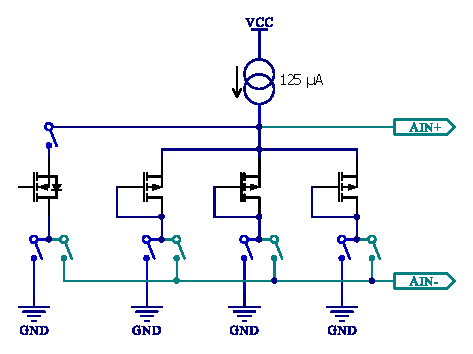
\includegraphics[width=0.7\paperwidth]{img/06/CD4007_mux_schematic.eps}
        \caption{Block diagram}
        \label{sensor_block_diagram}
    \end{figure}

\section{Low-level requirements}
    Using design requirements \ref{Design_requirements} and characteristic curves from \ref{Characteristic_curves} low-level specifications were listed:
    \begin{itemize}
        \item operating temperature range: $0 \div 60 \si{\degreeCelsius}$,
        \item compensated threshold voltage stability: \SI{\pm 0.5}{\milli\volt},
        \item current source value: $\SI{125}{\micro\ampere} \pm \SI{50}{\nano\ampere}$,
        \item ADC resolution: \SI{0.1}{\milli\volt} @ \SI{5}{\volt} reference = \SI{16}{bit}
    \end{itemize}


\section{Analog front-end}
    In this section decision and schematic diagrams of building blocks are presented.

    \subsection{SPICE models}
        Design should be validated by simulation. In this thesis, LTSpice XVII was used.

        Models used during simulation:
        \begin{itemize}
            \item CD4007 - model RIT4007P7 from Rochester Institute of Technology \cite{RIT_FULLER},
            \item Linear Technology components are embedded in LTSpice,
            \item other devices were modelled by hand using datasheets
        \end{itemize}

    \subsection{Linear regulator}
        Positive rail $+\SI{5}{V}$ on PC-104 stack comes from EPS, more specifically, this voltage is generated by a DC-DC converter (with \SI{500}{\kilo\hertz} switching frequency). Because of low noise requirements, the analog supply voltage has to be very well regulated and filtered. Because $V_{TH}$ of transistor will increase with absorbed dose, dropout from \SI{5}{\volt} should be as low as possible. As a tradeoff between this requirement and the available solutions on the market, analog rail voltage was chosen to be \SI{4.7}{\volt}.

        As an LDO regulator LT3042 was selected. It is ultralow noise, ultrahigh PSRR RF linear regulator by Linear Technology. Key specs \cite{LT3042_datasheet}:
        \begin{itemize}
            \item ultralow noise \SI{0.8}{\micro\volt RMS} (\SI{10}{\hertz} to \SI{100}{\kilo\hertz}),
            \item output current \SI{200}{\milli\ampere}
            \item input range \SI{1.8}{\volt} to \SI{20}{\volt}, output range \SI{0}{\volt} to \SI{15}{\volt}
            \item ultrahigh PSRR \SI{79}{\decibel} at \SI{500}{\kilo\hertz}, more detailed graph is shown in the figure \ref{LT3042_PSRR}.
            \item low dropout voltage of \SI{200}{\mV}
        \end{itemize}

        \begin{figure}[H]
            \centering
            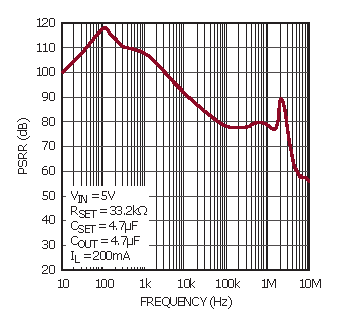
\includegraphics[width=0.4\paperwidth]{img/06/LT3042_PSRR.eps}
            \caption{LT3042 PSRR. Source: \cite{LT3042_datasheet}}
            \label{LT3042_PSRR}
        \end{figure}

        Thanks to this regulator, the conducted susceptibility requirement was met (\SI{175}{\mV} input ripple is cut down to \SI{19}{\uV}, which is enough for ADC to filter).

    \subsection{RadFET power switch}
        Because the main PLD microcontroller is also controlling the other sensors (photodiodes, temperature sensors), the RadFET analog front-end has to have the possibility to be turned off. For this purpose, the TPS2551DBVx current-limited power-distribution switch was implemented in the design.

        More accurately, two of them were implemented - one to disable the digital part of ADC and the second to disable all analog parts of the design.

        Apart from possibility of isolating the RadFET they provide point-of-load latch-up current limitation, allowing an ability to cut down the power in case of SEE even faster.

    \subsection{Current source}
        The current source has to be the most accurate part of the design, because the measured voltage depends on the square of its variation. It was assumed that $\SI{50}{\nano\ampere}$ current stability across temperature and aging range would be sufficient. The current source has to supply both the MOSFET (static resistance at operating point of about $20-25$~\si{\kilo\ohm}) and the body diode temperature sensor (static resistance at operating point of about     $3-7$~\si{\kilo\ohm})

        The main concept of the current source is based on the Burr-Brown application note \cite{Make_a_precision_current_source_or_sink}. The idea schematic is shown in the figure \ref{current_source_schematic}.

        \begin{figure}[H]
            \centering
            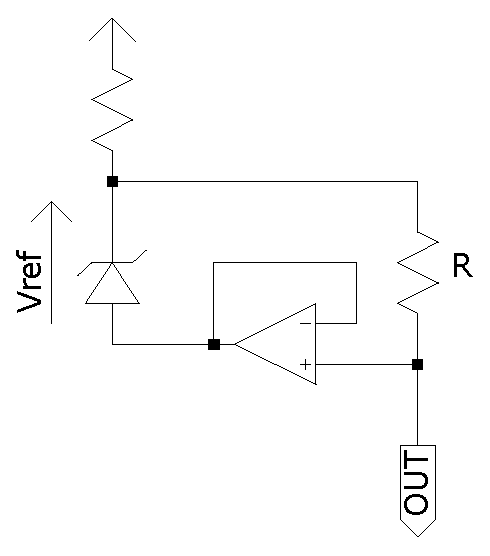
\includegraphics[width=0.3\paperwidth]{img/06/current_source_schematic.eps}
            \caption{Threshold voltage readout block diagram}
            \label{current_source_schematic}
        \end{figure}

        Output current is set by shunt voltage reference and resistor $R$, given by equation:
        $$I_{OUT} = V_{ref}/R$$

        Therefore, stability of output current depends on reference voltage and resistor accuracy.

        \bigskip \textbf{Shunt reference}

        After irradiation MOSFET $V_{DS}$ is planned to be no more than \SI{2.5}{\volt}, so the reference voltage has to be lower than \SI{2}{\volt}.

        Linear Technology LT1634-1.25 shunt voltage reference was chosen. It is one of the best shunt references from Linear Technology. Basic specification:
        \begin{itemize}
            \item \SI{0.05}{\percent} initial accuracy,
            \item \SI{10}{ppm/\degreeCelsius} maximum temperature drift,
            \item $< \SI{1}{\ohm}$ dynamic resistance,
            \item \SI{10}{\uA} minimal regulation current
        \end{itemize}

        Shunt resistance was chosen to make minimal current flowing through shunt reference large enough for specified loads - final value of \SI{5}{\kilo\ohm}.

        \bigskip \textbf{Series resistor}

        The value of this resistor reflects the required current flowing through the MOSFET. The nominal value selected was \SI{10}{\kilo\ohm}.

        The stability of this resistor across a temperature range is critical because it directly changes output current. To achieve the specified requirement, a \SI{10}{\kilo\ohm} / \SI{5}{ppm} resistor was chosen (APC0603T10K0Z).

        The manufacturer does not specify the exact value and profile of the temperature coefficient - so both worst cases were simulated (\SI{-5}{ppm} and \SI{5}{ppm}).

        \bigskip \textbf{Operational amplifier}

        The operational amplifier in this circuit should have very low bandwidth (noise limitation), low offset voltage (precision) and a small footprint. LTC2054 was selected - key characteristics:
        \begin{itemize}
            \item \SI{3}{\micro\volt} offset voltage,
            \item common mode $\pm \SI{0.5}{\volt}$ input/output range,
            \item \SI{500}{\kilo\hertz} gain-bandwidth product,
            \item device in Military Plastic package (temperature range $-55 \div \SI{150}{\degreeCelsius}$)
        \end{itemize}

        \bigskip \textbf{Simulation}
        Behavioral simulations were performed to find all possible problems with the circuit:
        \begin{itemize}
            \item temperature dependency,
            \item output resistance range,
            \item noise and stability
        \end{itemize}

        MOSFET/diode was replaced by a resistor emulating its static resistance ($\SI{2}{\volt}/\SI{125}{\micro\ampere} = \SI{16}{\kilo\ohm}$, $\SI{0.6}{\volt}/\SI{125}{\micro\ampere} = \SI{5}{\kilo\ohm}$, respectively). Simulation view is shown in the figure \ref{current_source_simulation}.

        \begin{figure}[H]
            \centering
            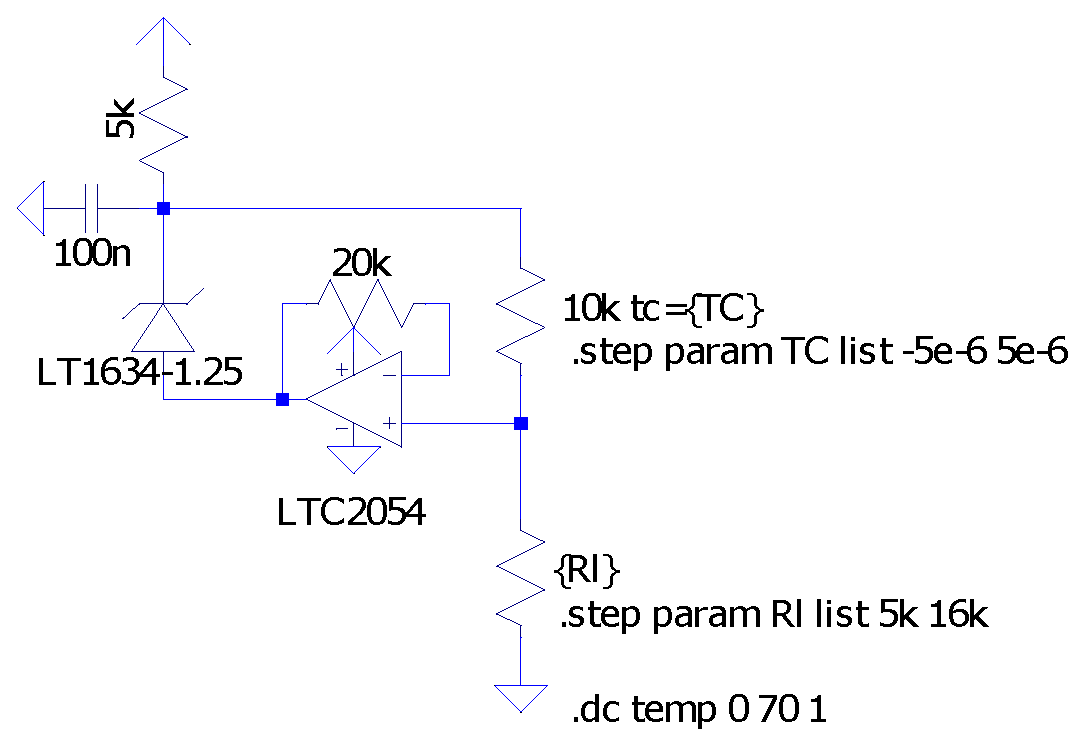
\includegraphics[width=0.5\paperwidth]{img/06/current_source.eps}
            \caption{Current source simulation}
            \label{current_source_simulation}
        \end{figure}

        \bigskip\textbf{Temperature dependency}
        Output current is shown in figure \ref{current_source_simulation_result}, simulation was performed on two different loads and resistor temperature coefficients.
        \begin{figure}[H]
            \centering
            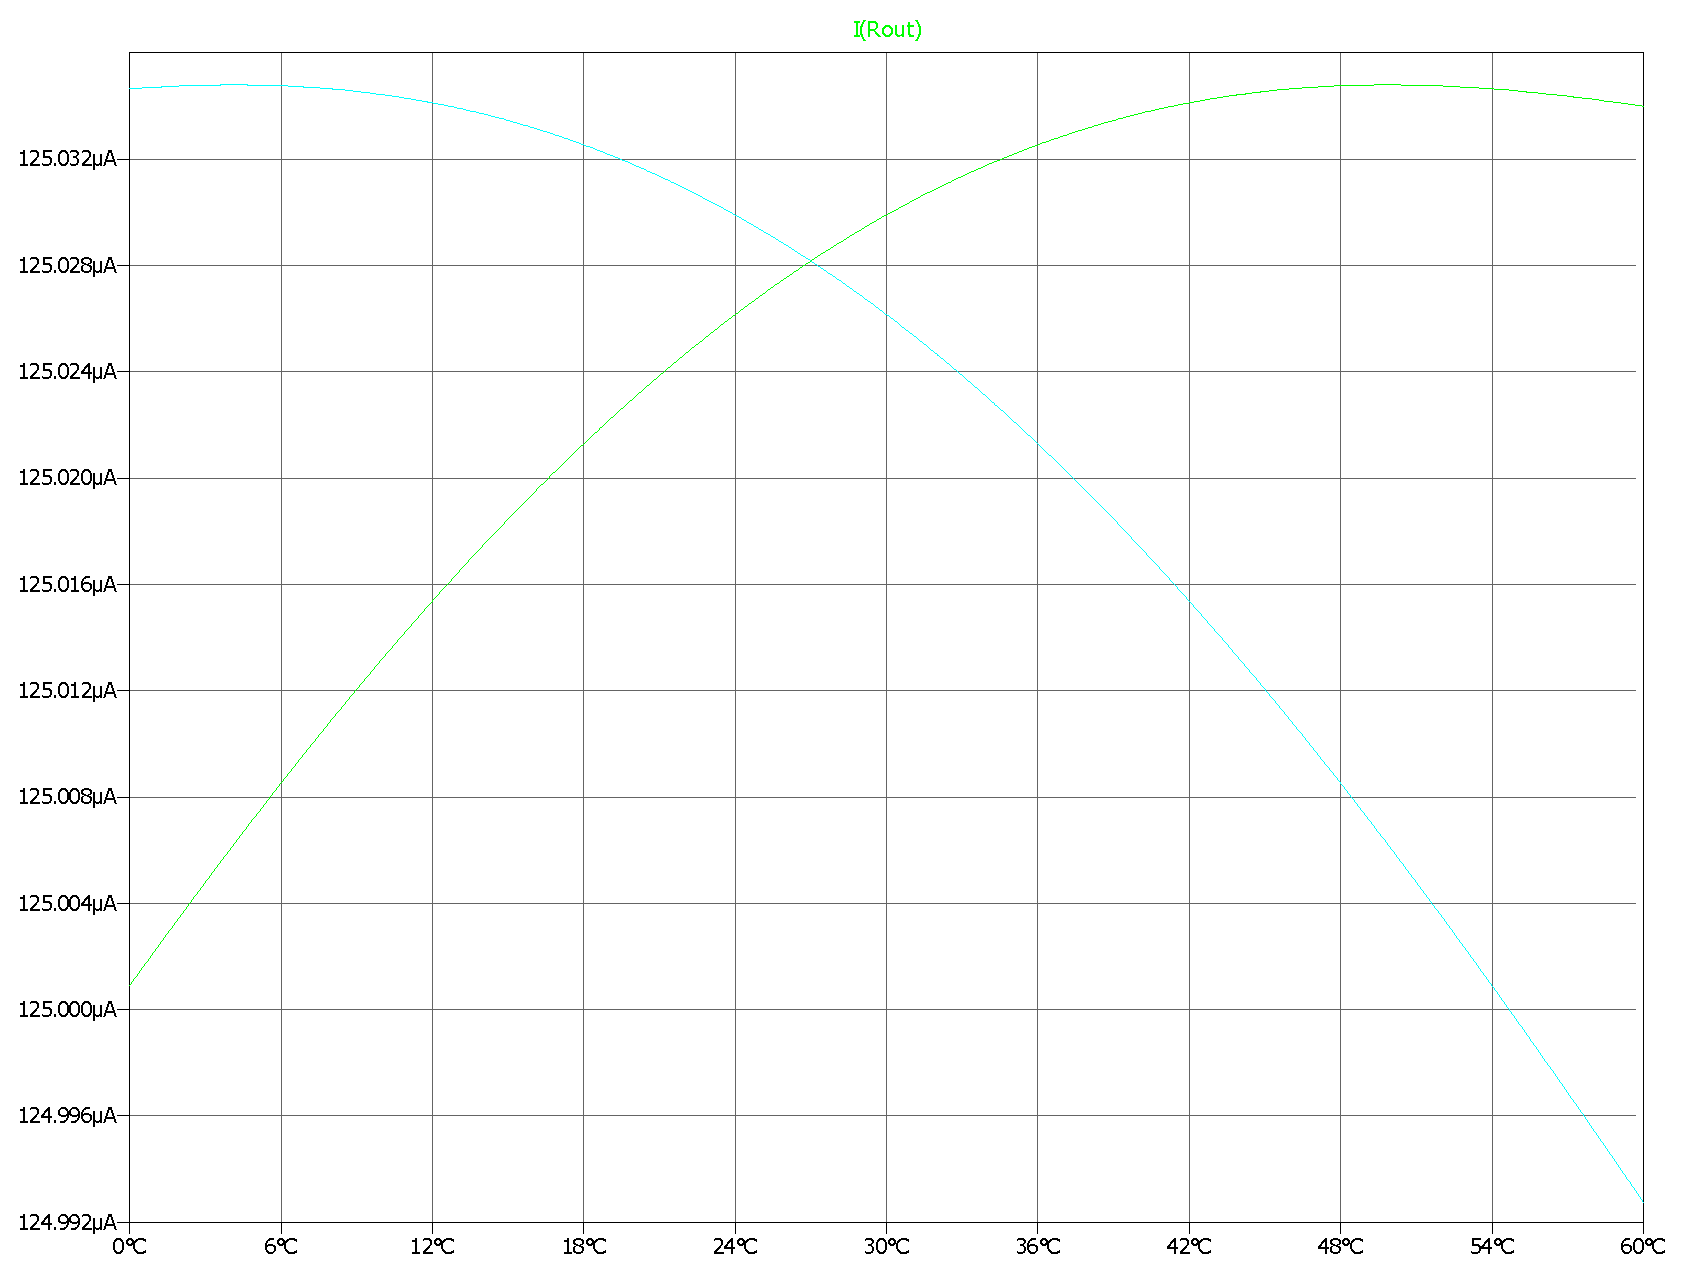
\includegraphics[width=0.8\paperwidth]{img/06/current_source_result.eps}
            \caption{Current source simulation result - output current}
            \label{current_source_simulation_result}
        \end{figure}

        In both cases, output current across temperature range does not exceed \SI{40}{\nano\ampere}.

        \bigskip\textbf{Output resistance range}
        \bigskip\textbf{Noise density}
        \bigskip\textbf{Stability}

    \subsection{Analog to digital converter}
        The analog to digital converter is responsible for reading $V_{DS}$ voltage across the transistor and voltage across the diode. Due to very low changes, high accuracy and resolution is required. Additionally, complex mixed signal elements like ADC should be radiation tested to prove long term reliability. To achieve at least \SI{0.1}{\milli\volt} resolution, ADC has to be at least \SI{16}{bits}.

        Due to constraints on the system and reliability issues, the AD7714 from Analog Devices was chosen. Radiation tests have shown that it fails between \SI{10}{\kilo\rad} and \SI{20}{\kilo\rad}, with no degradation up to \SI{10}{\kilo\rad} \cite{ADC_radiation_tests}.

        Internal diagram is shown in figure \ref{AD7714}. Key specs:
        \begin{itemize}
            \item \SI{24}{bits},
            \item \SI{0.0015}{\percent} nonlinearity,
            \item programmable gain ($1 \div 128$),
            \item 3 fully differential or 5 pseudo-differential input channels
            \item \SI{3}{\volt} or \SI{5}{\volt} operation
            \item separated digital and analog supply and grounds,
            \item SPI interface
            \item \SI{0.25}{\hertz} sampling frequency for strongest filter,
        \end{itemize}

        \begin{figure}[H]
            \centering
            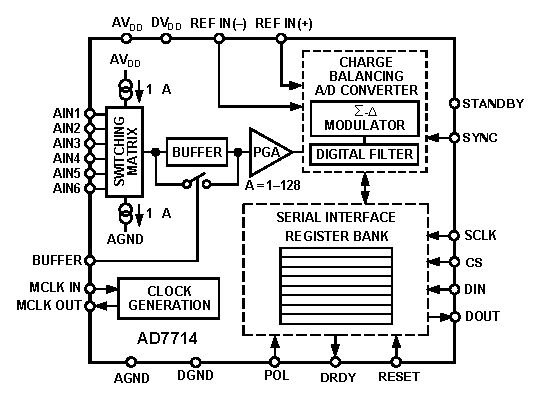
\includegraphics[width=0.5\paperwidth]{img/06/AD7714.eps}
            \caption{AD7714 internal block diagram. Source: \cite{AD7714_datasheet}}
            \label{AD7714}
        \end{figure}

        AD7714 requires external crystal or clock oscillator in the frequency range \SI{1}{\mega\hertz} to \SI{2.54}{\mega\hertz}. Crystal oscillators for these frequencies are large and susceptible to shocks and damage because of their large, delicate internal structure (firure \ref{Opening_a_Quartz_Crystal_Can_Effects_Thereof}). \SI{1}{\mega\hertz} ceramic oscillator ISM95-3351AH was therefore selected for operation (figure \ref{ISM95-3351AH-1.0000}).

        \begin{figure}[H]
            \centering
            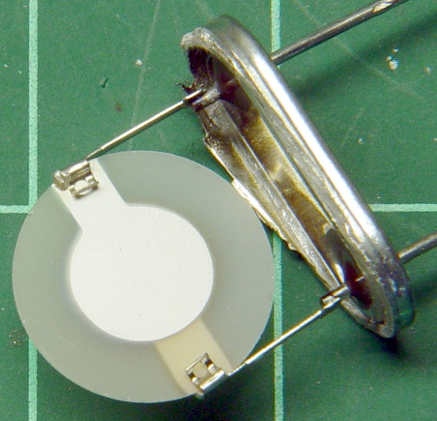
\includegraphics[width=0.5\paperwidth]{img/06/crystal.png}
            \caption{Low frequency crystal oscillator internals. Source: \cite{Opening_a_Quartz_Crystal_Can_Effects_Thereof}}
            \label{Opening_a_Quartz_Crystal_Can_Effects_Thereof}
        \end{figure}

        \begin{figure}[H]
            \centering
            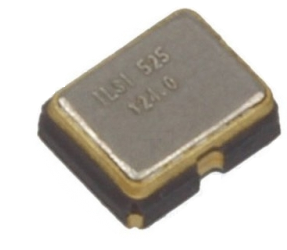
\includegraphics[width=0.5\paperwidth]{img/06/ISM95.png}
            \caption{ISM95-3351AH-1.0000 ceramic oscillator package. Source: \cite{ISM95_series_datasheet}}
            \label{ISM95-3351AH-1.0000}
        \end{figure}


    \subsection{Multiplexer}
        The multiplexer has two purposes: to multiplex current and voltage lines (3-wire readout).

        As an analog multiplexer, ADG709 was chosen. Its radiation tests can be found in \cite{IEEE_radiation_tests_1992_2009}. It is a double 1:4 mux, allowing for simultaneous current and voltage multiplexing. It's internal block diagram is shown in figure \ref{ADG709_block}

        \begin{figure}[H]
            \centering
            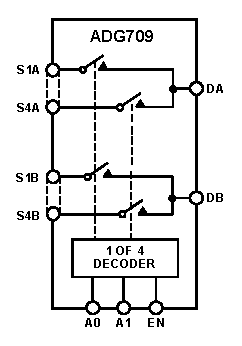
\includegraphics[width=0.3\paperwidth]{img/06/ADG709.eps}
            \caption{ADG709 internal block diagram. Source: \cite{ADG709_datasheet}}
            \label{ADG709_block}
        \end{figure}

        Due to ESD diodes in CD4007, an additional current switch had to be added to cut off potential from n-MOS body diode. For this purpose, a simple 1-channel analog switch ADG849YKSZ was implemented.

    \subsection{Differential \& common mode filter}
        The internal sampling frequency of ADC (for GAIN = 1 and $f_{clk} = \SI{1}{\mega\hertz})$ is about \SI{15.6}{\kilo\hertz}. To eliminate aliasing and reduce readout noise, a low-pass differential filter should be implemented on ADC input.

        A simple one-pole RC filter was selected. Its schematic can be found in the figure \ref{low_pass_filter}.

        \begin{figure}[H]
            \centering
            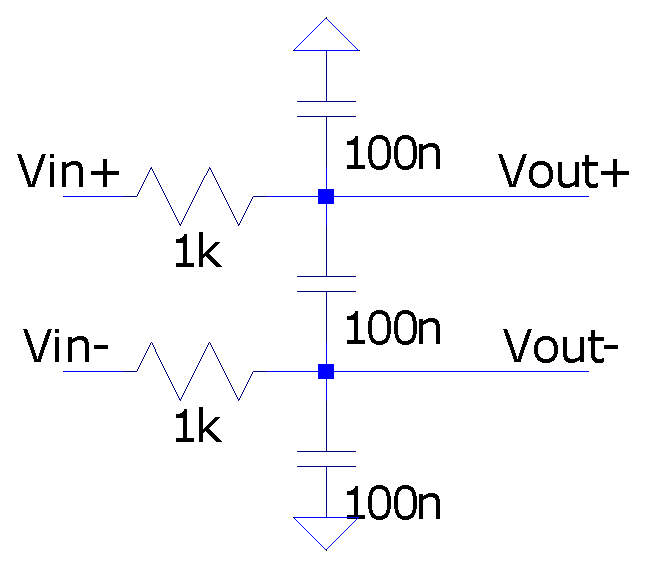
\includegraphics[width=0.3\paperwidth]{img/06/low_pass_filter.eps}
            \caption{Low pass filter schematic.}
            \label{low_pass_filter}
        \end{figure}

        Using AC analysis it's frequency characteristic was obtained - figure \ref{low_pass_filter_output}. At half the sampling frequency, attenuation is about \SI{22}{\decibel}.

        \begin{figure}[H]
            \centering
            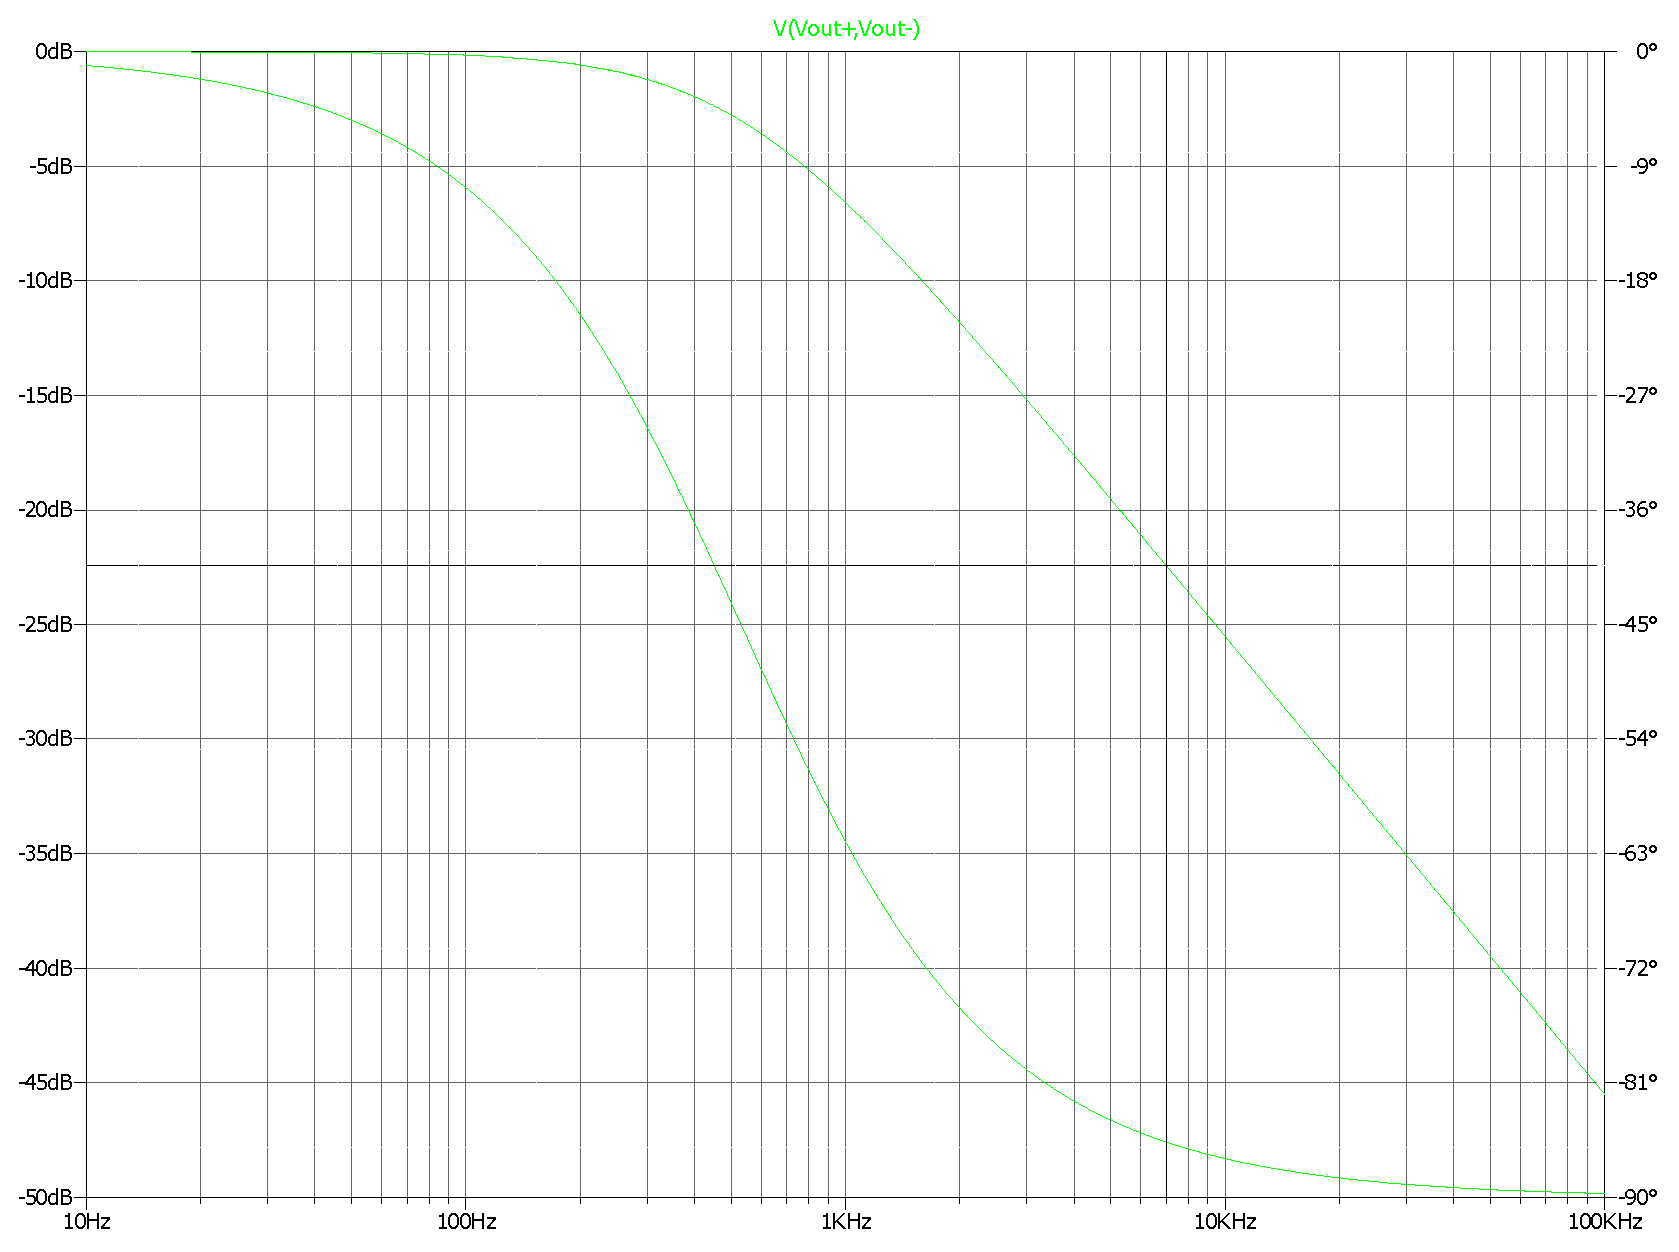
\includegraphics[width=0.7\paperwidth]{img/06/low_pass_filter_output.eps}
            \caption{Low pass filter frequency characteristics.}
            \label{low_pass_filter_output}
        \end{figure}

    \subsection{Shielding}
        Because of noise requirements and near proximity of \SI{0.5}{\watt} radio transmitter, EMI shielding was tested.

        Proper pads for EMI shielding were placed on PCB. Its size depends on PCB layout, after routing it was decided to use the BMI-S-203 shield (figure \ref{BMI-S-203}). This shield should provide attenuation of about \SI{50}{\decibel} at the transmitter frequency.

        \begin{figure}[H]
            \centering
            
\includegraphics[width=0.7\paperwidth]{img/06/BMI-S-203.eps}
            \caption{BMI-S-203 shield. Source: \cite{EMI_shieldings_catalog}}
            \label{BMI-S-203}
        \end{figure}


\section{Digital}
    RadFET is mainly an analog sensor. However, LDO, MUX and ADC have to be controlled from the on-board microcontroller. On the other hand, the RadFET has to be accessible from OBC, to retrieve data and send them to the ground station.

    \subsection{Microcontroller}
        The main digital part of the design is the microcontroller. It will be responsible for:
        \begin{itemize}
            \item controlling analog part of the sensor,
            \item implementing FDIR in case of any failure,
            \item communicating with OBC to retrieve data.
        \end{itemize}

        Several options were considered, and the final choice was ATmega164PV-10AQ. More detailed comparison can be found in \cite{PWSAT_EPS_CDR}.

        AVR devices are known for their simplicity, reliability and sparsity of bugs. Radiation tests were performed for ATmega series, showing their performance for up to \SI{30}{\kilo\rad} \cite{ATMEGA128_radiation_tests}.

        Features of this particular device:
        \begin{itemize}
            \item \SI{1.8}{\volt} - \SI{5.5}{\volt} supply voltage,
            \item \SI{4}{\mega\hertz} clock,
            \item TQFP-44 package,
            \item \SI{16}{\kilo B} program memory,
            \item \SI{1}{\kilo B} SRAM
        \end{itemize}

    \subsection{On-Board Computer interface}
        The interface to OBC is $I^2C$ bus. Because the sensor can be turned off by cutting its voltage, proper buffering had to be implemented. For this purpose $I^2C$ repeater PCA9517 was placed between OBC and the in-sensor microcontroller. Its functional diagram can be seen in figure \ref{PCA9517}. From it's datasheet: "The SDA and SCL pins are over voltage tolerant and are high-impedance when the PCA9517 is unpowered." \cite{PCA9517_datasheet}. Thanks to this, OBC can completely disable the sensor by simply cutting off power.

        \begin{figure}[H]
            \centering
            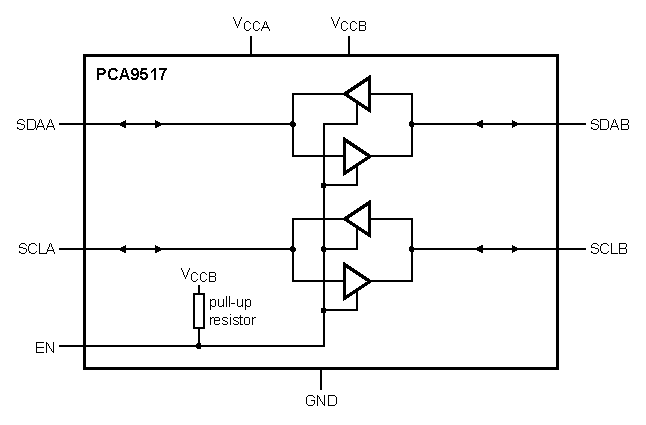
\includegraphics[width=0.7\paperwidth]{img/06/PCA9517.eps}
            \caption{PCA9517 internal block diagram. Source: \cite{PCA9517_datasheet}}
            \label{PCA9517}
        \end{figure}


\section{Final schematic}
    The top level schematic file can be seen in figure \ref{top_level_schematic}. Ports represent physical connectors - to satellite bus and debug socket.

    \begin{figure}[H]
        \centering
        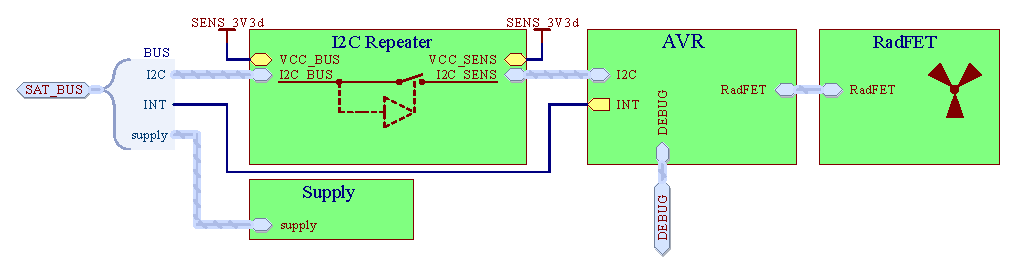
\includegraphics[width=0.8\paperwidth]{img/06/final_schematic_top.eps}
        \caption{Top level schematic}
        \label{top_level_schematic}
    \end{figure}

    "RadFET" makes up the analog part of the design. Its block diagram can be seen in figure \ref{analog_schematic}.

    \begin{figure}[H]
        \centering
        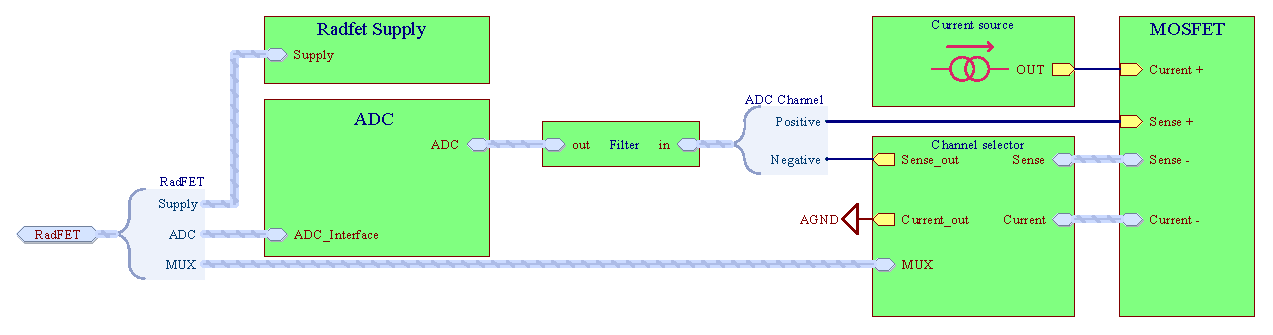
\includegraphics[width=0.8\paperwidth]{img/06/final_schematic_radfet.eps}
        \caption{Sensor final schematic - analog part}
        \label{analog_schematic}
    \end{figure}


\section{PCB}
    The engineering model of the sensor was manufactured on a similar board to the flight model. It should represent the space required for this sensor, noise coupling and performance.

    For schematic capture, PCB layout and DRC Altium Designer EDA software was used.

    \subsection{PCB materials}
        During the initial phase of the PW-Sat2 project it was decided that all self-made boards would be manufactured from FR4 laminate. Because most space-qualified PCBs are made of polyimide, it is very hard (and expensive) to manufacture them. Apart from a higher glass transition temperature they do not provide many advantages.

        Care should be taken to check for:
        \begin{itemize}
            \item vibration tolerance,
            \item gluing quality of multiple layer boards,
            \item outgassing coefficient.
        \end{itemize}

        With this in mind, a manufacturer of PCB was selected - Technoservice S.A.

    \subsection{PCB stack}
        Because outgassing of devices can be dangerous for turbomolecular pumps, it must be limited as much as possible. Therefore soldermask and overlay layers are not present in the design, and packages of used components have known outgassing coefficients.

        Although this prototype board has 4 layers, the on flight model board will be 6-layered. The PCB stack generated from Altium Designer is shown in figure \ref{PCB_Altium_stack}.

        \begin{figure}[H]
            \centering
            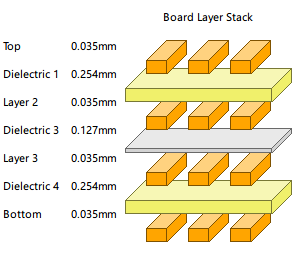
\includegraphics[width=0.3\paperwidth]{img/06/stack.png}
            \caption{Sensor PCB stack}
            \label{PCB_Altium_stack}
        \end{figure}

    \subsection{PCB layout}
        The PCB layout in the mixed signal board is very important. Ground potential shifts, induced noise, coupling between ground planes - all these effects were considered during the layout process.

        \bigskip \textbf{Top \& bottom layers}

        Components should be placed only on top and bottom layers, every net should be connected on internal layers. Because the model exists only on a 4-layer board this design recommendation is not fulfilled - this will be forced on Flight Model. Final layout is shown in figure \ref{top_bottom_layer_layout}.

        \begin{figure}[H]
            \centering
            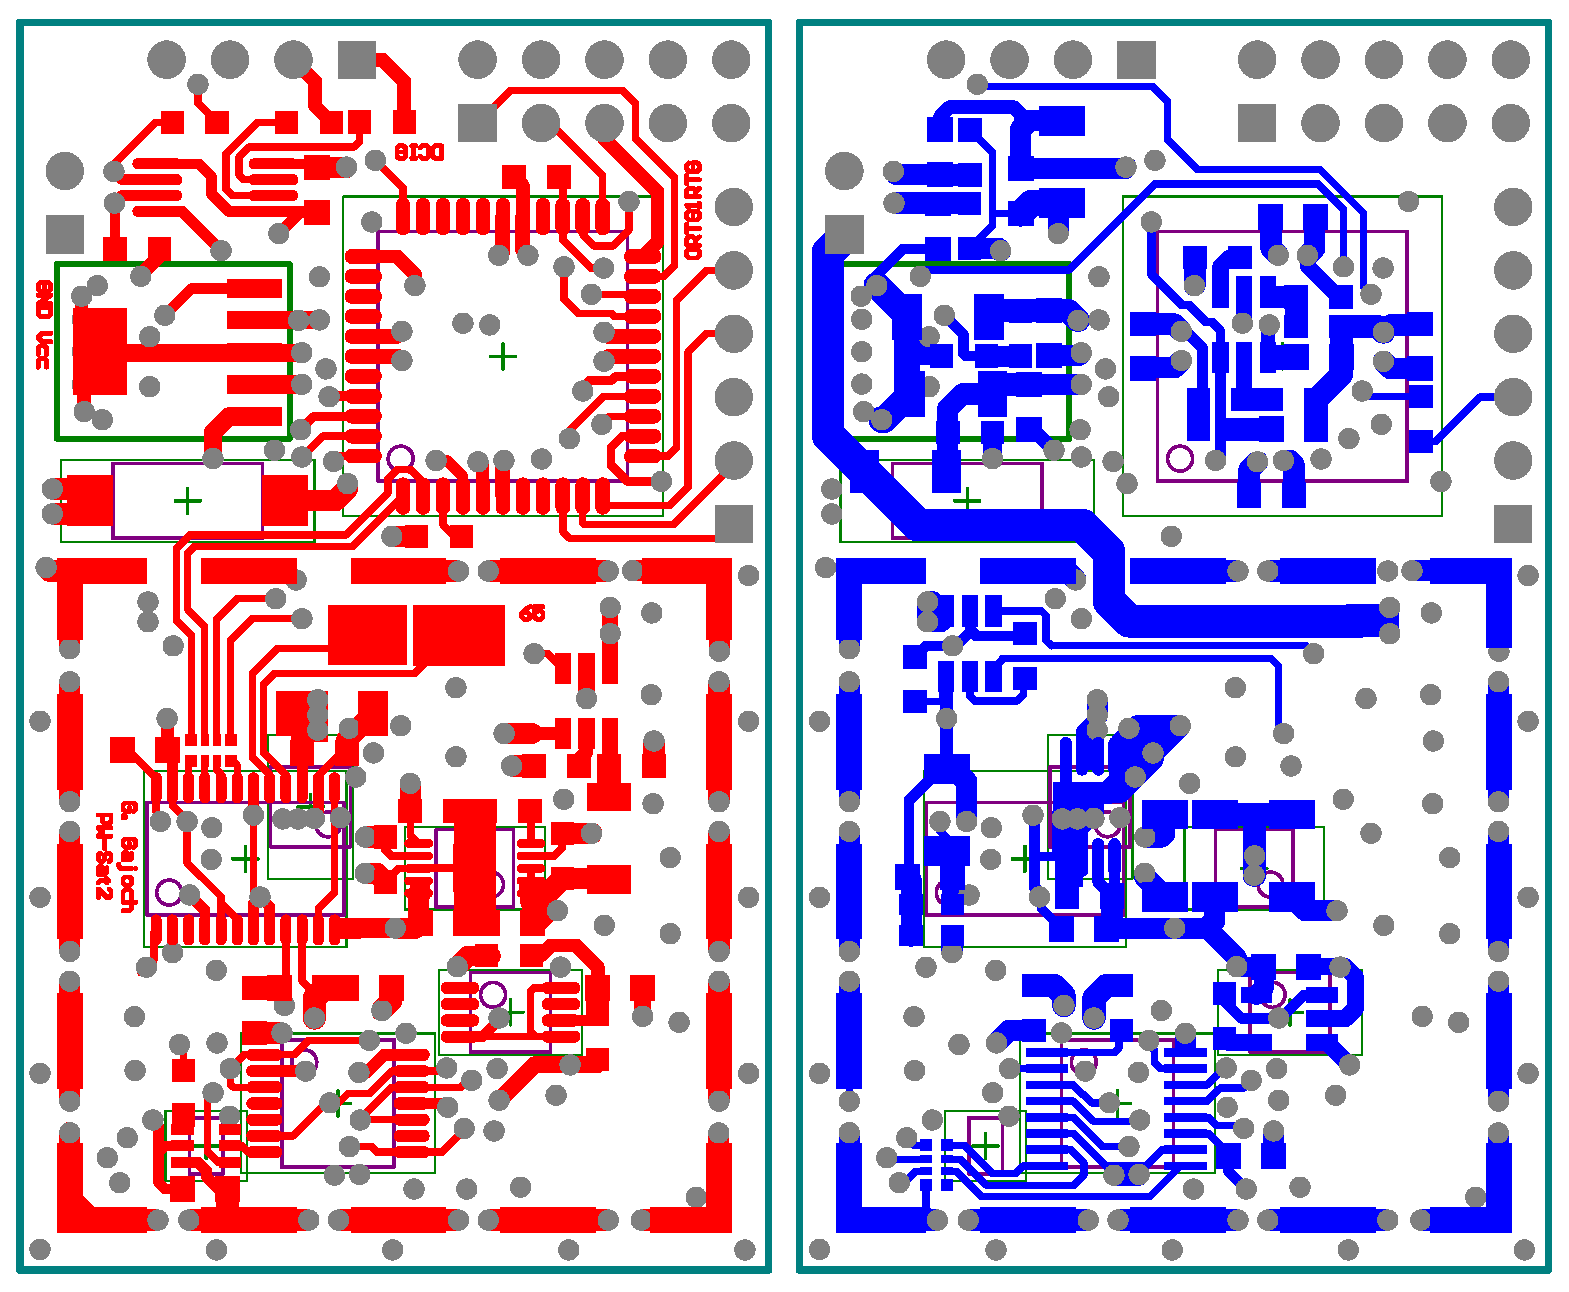
\includegraphics[width=0.5\paperwidth]{img/06/top_bottom_layer_layout.eps}
            \caption{Top and bottom layer layout}
            \label{top_bottom_layer_layout}
        \end{figure}

        \bigskip \textbf{Internal layers}

        One layer of the board was designed to serve completely as a ground plane. More specifically, two ground planes - an analog and a digital one, connected under ADC. The second internal layer provides routing space, but also has ground planes on it (due to PCB temperature bending, the PCB cannot have only one ground plane). Layout is shown in figure \ref{internal_layers_layout}.

        \begin{figure}[H]
            \centering
            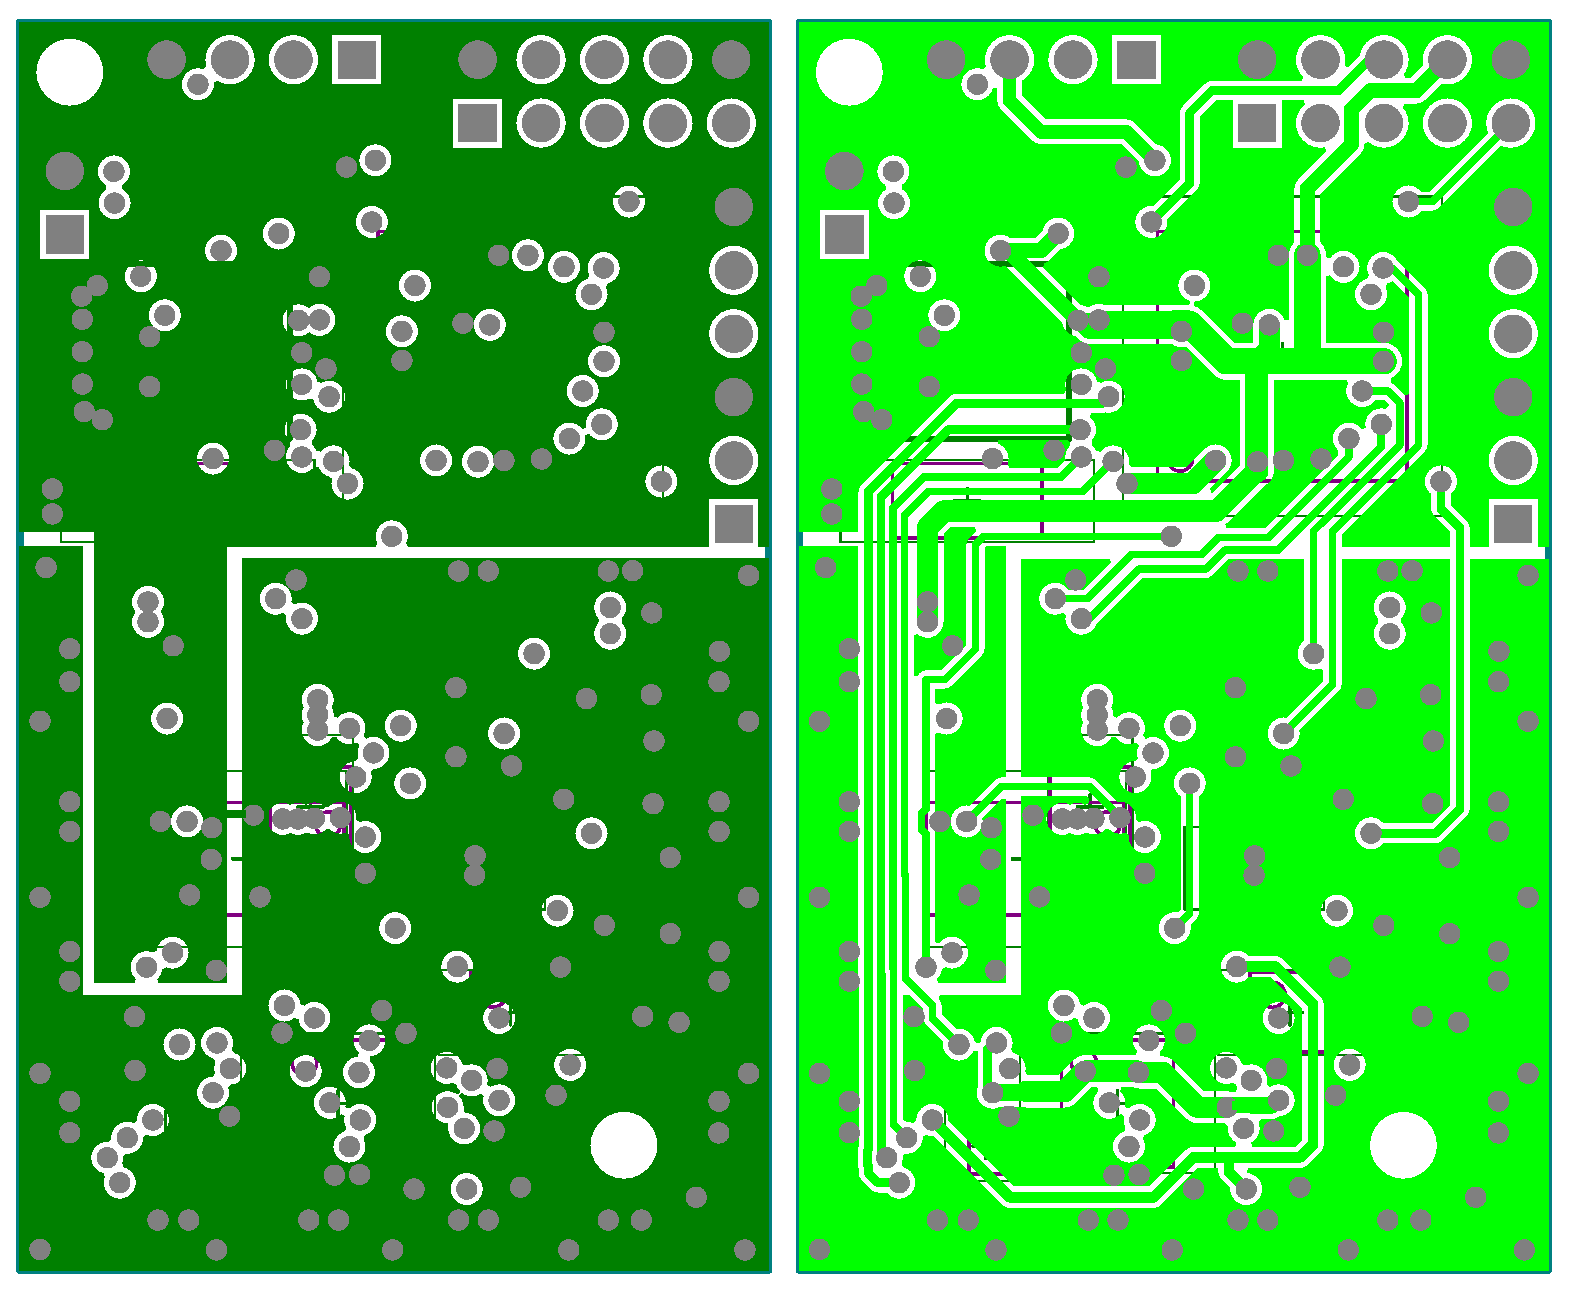
\includegraphics[width=0.5\paperwidth]{img/06/internal_layers_layout.eps}
            \caption{Internal layers layout}
            \label{internal_layers_layout}
        \end{figure}

    \subsection{3D model}
        Using the Altium designer and proper self-made libraries, a 3D model of board can be easily generated. In figure \ref{pcb_3d_model} a 3D model with and without EMI shielding is shown.

        \begin{figure}[H]
            \centering
            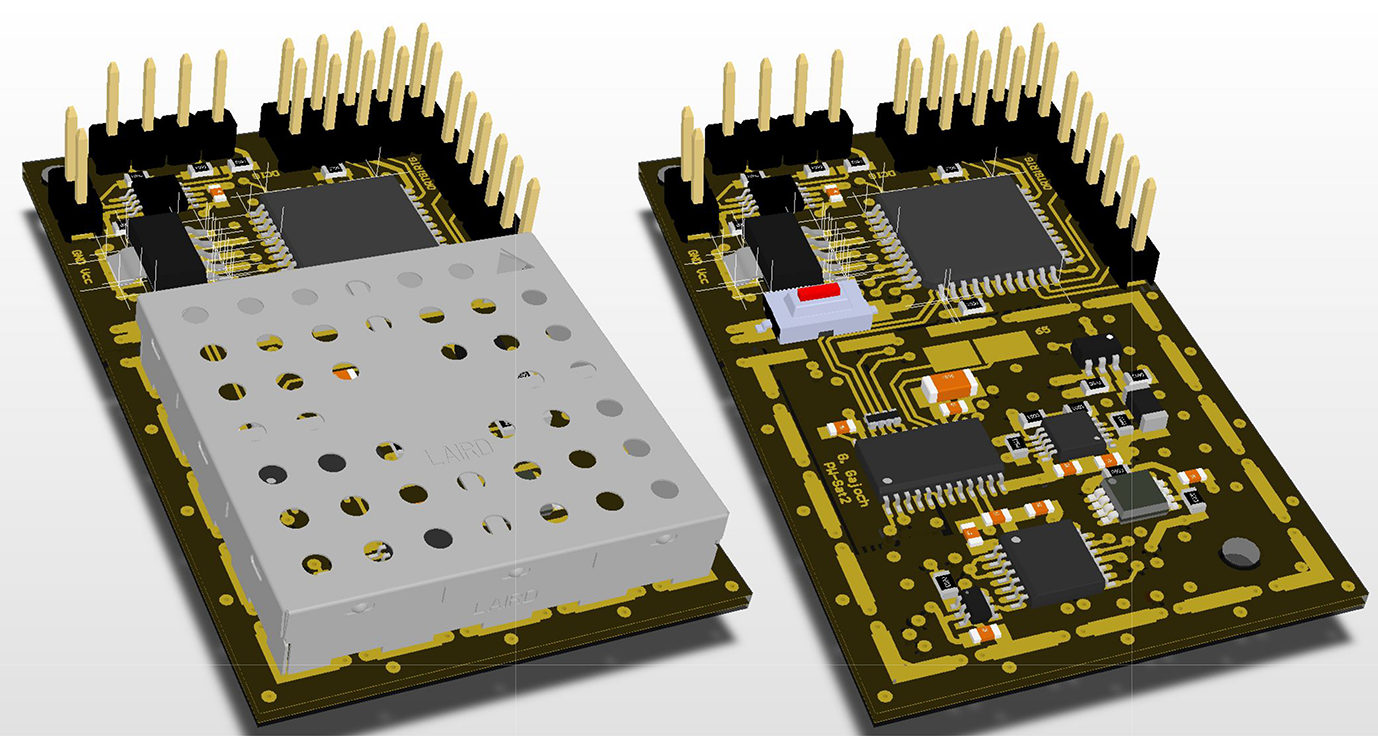
\includegraphics[width=0.8\paperwidth]{img/06/pcb_3d_model.png}
            \caption{3D view of engineering model with and without EMI shield}
            \label{pcb_3d_model}
        \end{figure}

\section{Software design}
    An important aspect of the sensor is it's embedded software. It has to control data acquisition (LDO, ADC, MUX), check for validity and expose \iic interface to OBC.

    Because the main microcontroller is 8-bit AVR-core processor, software has to be highly optimized, especially for speed and data memory consumption. Available resources:
    \begin{itemize}
        \item \SI{16}{\kilo B} of FLASH,
        \item \SI{1}{\kilo B} of SRAM,
        \item \SI{1}{\mega\hertz} clock frequency.
    \end{itemize}

    Software for the sensor was written in C++14, using the AVR-HAL library developed by the PW-Sat2 team. A schematic of software building blocks is shown in figure \ref{Sensor_software_diagram}.

    \begin{figure}[H]
        \centering
        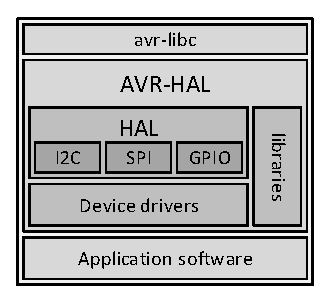
\includegraphics[width=0.5\paperwidth]{img/06/software_diagram.eps}
        \caption{Sensor software diagram}
        \label{Sensor_software_diagram}
    \end{figure}

    \subsection{AVR-HAL}
    AVR-HAL is a library created to ease software development on AVR microcontrollers. It was created by the PW-Sat2 team, with low overhead (in most modules zero-data usage), extensibility and modern software development languages and techniques (C++14, unit and integration testing) in mind. It was created for a specific purpose: embedded software development on-board PW-Sat modules (EPS, PLD, SunS). Therefore, only a few devices are officially supported (ATmega164, 165, 328), with extensible tests on existing platforms.

    AVR-HAL consists of basic modules:
    \begin{itemize}
        \item C++14 libraries not existing in avr-libc (type traits, array, array\_view),
        \item Hardware Abstraction Layer - identical low-level API for every ported device,
        \item Device Drivers - drivers for many used integrated circuits used on PW-Sat2,
        \item Debugging libraries - software created to allow unified debugging of many devices (serial port, command line interface, gdb connection etc).
    \end{itemize}

    Using AVR-HAL, writing application software is only high-level work, leaving all hardware access to the tested and proven library.

    \subsection{$I^2C$-slave interface}
    Cubesat standards define two \iic lines along the satellite board stack, which most of the commercially available devices use. It was the easiest option for connecting the PLD board to OBC, so this communication bus was selected.

    The sensor acts as a slave on the \iic bus. Communication protocol is based on a request-reply manner, with the interrupt pin state acting as a notification.

    When OBC wants to gather data from the sensor it will do following tasks in order:
    \begin{itemize}
        \item send measurement start request to sensor (table \ref{Start_measurement_command}),
        \item wait until conversion is completed (pulse on interrupt line is triggered),
        \item read data from sensor internal memory (table \ref{Data_readout_command}).
    \end{itemize}

    \begin{table}[H]
        \begin{center}
            \begin{tabular}{|c|c|c|c|}
                \hline
                START & 0x20+W & 0x80 & STOP \\ \hline
            \end{tabular}
        \end{center}
        \caption{Start measurement command}
        \label{Start_measurement_command}
    \end{table}

    \begin{table}[H]
        \begin{center}
            \begin{tabular}{|c|c|c|c|c|c|c|}
                \hline
                START & 0x20+W & 0x00 & REP-START & 0x20+R & (...data...) & STOP \\ \hline
            \end{tabular}
        \end{center}
        \caption{Data readout command}
        \label{Data_readout_command}
    \end{table}

    \subsection{Measurement algorithm}
    \bigskip \textbf{RadFET sensor}

    The sensor, after receiving "start measurement" command (table \ref{Start_measurement_command}) does following steps:
    \begin{itemize}
        \item enable LDO,
        \item wait for power line stabilization,
        \item for each channel in [MOS0, MOS1, MOS2, TEMPERATURE]:
        \begin{itemize}
            \item[$\circ$] select proper MUX switch,
            \item[$\circ$] enable MUX,
            \item[$\circ$] wait for stabilization,
            \item[$\circ$] read ADC value,
            \item[$\circ$] disable MUX
        \end{itemize}
        \item disable LDO,
        \item make a positive pulse on interrupt line, informing OBC about conversion finish.
    \end{itemize}

    \bigskip \textbf{OBC}

    When OBC wants to read data from the sensor (issued by telecommand from ground station) it performs the following steps:
    \begin{itemize}
        \item enable PLD power by sending proper command to EPS,
        \item send "start measurement" command to RadFET,
        \item wait for trigger on interrupt line (external interrupt pin),
        \item send "data readout" command and store data in memory,
        \item disable power for PLD board
    \end{itemize}

\section{Assembly}
    For the final model, proper ECSS standards will be applied during soldering and integration. On the engineering model proper tools and techniques should be tested to eliminate unnecessary problems later on.

    Equipment used during soldering and integration is compliant with ECSS standards, the same tools are used on flight hardware:
    \begin{itemize}
        \item Weller WMRP station,
        \item \SI{63}{\percent} Sn/\SI{37}{\percent} Pb \SI{0.2}{\milli\meter} soldering wire,
        \item Alpha RMA - ROL0 flux,
        \item ESD-protected workstation and tools.
    \end{itemize}

\section{Finished sensor}
    Photo of sensor after integration can be seen in the figure \ref{Integrated_sensor}.

    \begin{figure}[H]
        \centering
        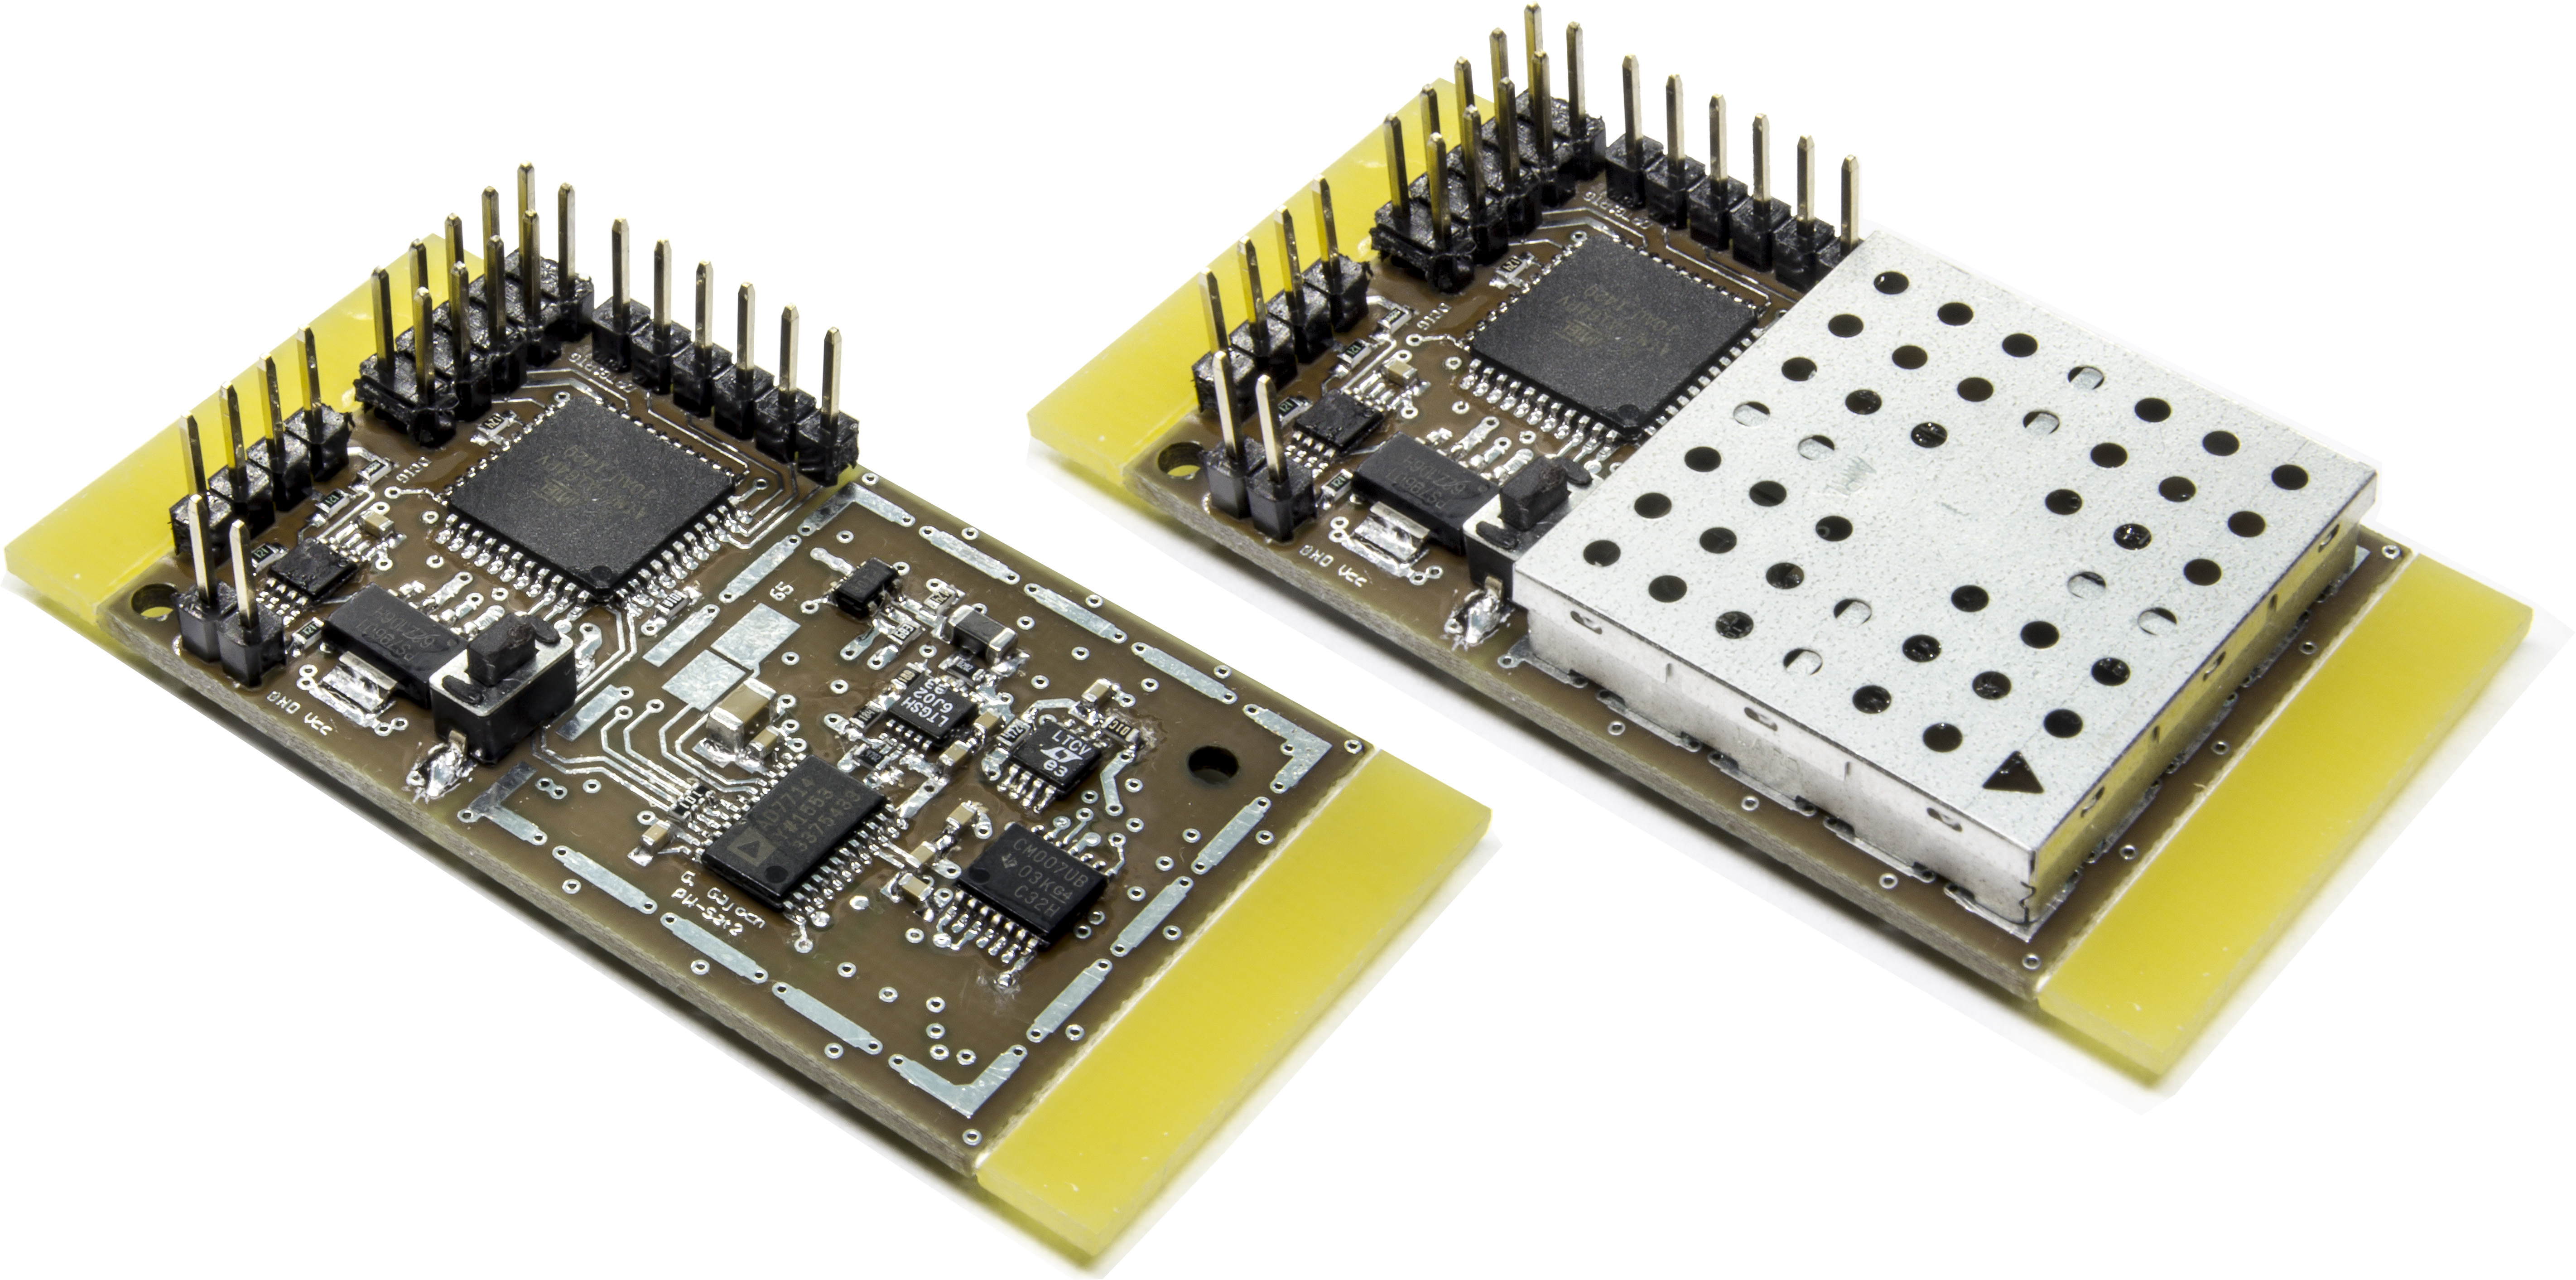
\includegraphics[width=0.8\paperwidth]{img/06/finishiedSensorPhoto.jpg}
        \caption{Integrated sensor without and with EMI shield}
        \label{Integrated_sensor}
    \end{figure}
